%SPDX-License-Identifer: CC-BY-SA-4.0
%License-Filename: LICENSE

\documentclass[a4paper]{article}

\usepackage[USenglish,ngerman]{babel}
\usepackage[utf8]{inputenc}
\usepackage[T1]{fontenc}
\usepackage{geometry}
\usepackage{lastpage}
\usepackage{amsmath}
\usepackage{listings}
\usepackage{hyperref}
\usepackage{graphicx}
\usepackage{acronym}
\PassOptionsToPackage{hyphens}{url}
\usepackage{hyperref}


\geometry{
	a4paper,
	top=25mm,
	left=25mm,
	right=25mm,
	bottom=13mm,
	headsep=4mm,
	footskip=7mm}
\title{Titel}
\author{Jochen Saalfeld}
\usepackage{fancyhdr}
\pagestyle{fancy}
\fancyhf{}
\fancyhead[L]{Konzeptpapier - Bachelorarbeit}
\fancyhead[C]{}
\fancyhead[R]{Jochen Saalfeld}
\renewcommand{\headrulewidth}{0.4pt}
\fancyfoot[C]{Seite \thepage ~von \pageref{LastPage}}
\renewcommand{\footrulewidth}{0.1pt}


\begin{document}
\section*{Vom herkömmlichen Applikationshosting Django basierter Anwendungen 
zur \acf{SaaS} am Beispiel von OpenSlides}
%Motivation und Einleitung, am besten halbwegs Laienverständlich
Die Bachelor Arbeit, die aus der beschriebenen Planung dieses Dokuments 
entsteht, wird bei der Intevation GmbH\cite{inte} geschrieben. Der Autor des 
Dokuments ist seit über 2 Jahren bei der Intevation GmbH angestellt und hat 
während seines Studiums dort gearbeitet. Die Intevation GmbH schreibt seit über 
18 Jahren freie Software mit freier Software, weswegen im Rahmen der 
Bachelorarbeit ausschließlich freie und/oder Quelloffene Software betrachtet 
wird. Unter anderem hat der Autor an Gpg4win\cite{gpg4win} und 
OpenSlides\cite{oshp} mitgewirkt.\\
\\
OpenSlides ist eine Django\cite{djangohp} basierte Web-Anwendung zur 
Unterstützung von 
Versammlungen. Mit der Software lassen sich mehrere Arbeitsabläufe abbilden, 
die bei der Verwaltung und Durchführung von Veranstaltungen unterstützen. 
OpenSlides bietet dabei unter anderem die Möglichkeit Redelisten, 
Tagesordnungen, Anträge und Wahlen zu leiten. Hierbei können alle beteiligten 
an einer Veranstaltung auf die Software zugreifen und damit in verschiedenen 
Rollen interagieren\cite{oshp}. Intevation GmbH bietet auch Support und Hosting 
für OpenSlides bei Veranstaltungen an\cite{oscom}.\\
\\
Beim herkömmlichen Applikationhosting ist aufgefallen, dass bei Veranstaltungen 
mit vielen Teilnehmern entsprechend viel Leistung beim Hosting der Applikation 
benötigen. Meist sind Veranstaltungen nur über einen beschränkten Zeitraum von 
wenigen Tagen. In diesen wenigen Tagen wird die gebotene Leistung gut genutzt. 
In den Wochen und Monaten der Vor- und Nachbereitung jedoch nicht. Hier wird 
jedoch die Möglichkeit gesehen durch eine Prozessvirtualisierung der Software 
die Leistung besser zu nutzen, um so das Angebot für den Kunden attraktiver zu 
gestalten und den Fußabdruck der nötigen durch geschickte Orchestrierung und 
Planung zu verkleinern.
\section{Stand der Technik} \label{sec:sdt}
%Wie sieht es gerade aus da draußen?
\subsection{Prozessvirtualisierung} \label{subsec:sdtpv}
Die Virtualisierung und die Nutzung von Software und Prozessen und die 
Ausgliederung von Abhängigkeitsmanagement in Container ist nicht erst ein Thema 
der letzten Jahre. Bereits 1979, als Unix in der Version 7 entwickelt wurde, 
wurde \texttt{chroot} eingeführt. Leider bietet es sich nicht für OpenSlides 
als Virtualisierung an, da chroot keine Root Privilegien Isolation 
unterstützt.\cite{containerhist}\\
\\
Zwischen 1972 und heute sind natürlich viele neue Tools hinzugekommen, die in 
irgend einer Art und Weise die Virtualisierung von Prozessen unterstützen. Es 
sollen jedoch nur jene betrachtet werden, welche die Spezifikationen der 
\acf{OCI}\cite{oci} unterstützen. Die \ac{OCI} hat sich im Jahre 2015 aus 
verschiedenen führenden Technologieanbietern im Bereich der Container basierten 
Virtualisierung gegründet um einen offenen Standard zu entwickeln. Dieser 
wird von den Technologieführern\cite{ocimembers} entwickelt und implementiert.
Im Rahmen der Betrachtung der Technolgien zur 
Prozessvirtualisierung werden nur Tools betrachtet, welche diesem Standard 
folgen. Diese Entscheidung wurde getroffen, da abzusehen ist, dass dieser 
Standard noch lange existiert und das auch über verschiedene Tools hinweg. Eine 
Zukunft ist also gesichert.\\
\\
Durch den Standard, der durch die \ac{OCI} gepflegt wird, unterscheiden sich 
die Produkte nur noch in einigen Punkten. So kann lediglich die 
Beschreibungssprache zum bereitstellen eines Containers als Image 
unterschiedlich sein.  Einmal erstellt, sind die Images jedoch durch jedes Tool 
nutzbar. Dann können die Images wiederum unterschiedlich durch die Werkzeuge 
behandelt werden. Den \glqq{}Rohling\grqq{} für einen Container, nennt man 
Image.\\
\\
Zur Zeit gibt es drei große Lösungen, welche den Richtlinien der \ac{OCI} 
folgen. Zum einen \texttt{rkt} (rock-it gesprochen), welches von den 
Entwicklern des Betriebssystems \grqq{}CoreOS\glqq{} im Jahre 2014 
veröffentlicht wurde\cite{rkthp}. Des weiteren gibt es seit kurzem 
\texttt{railcar} von \grqq{}Oracle\glqq{}, welches eine auf der 
Programmiersprache \texttt{rust} basierende Implementation des \ac{OCI} 
Standards ist\cite{railcarhp}. Abschließend gibt es \texttt{docker} von der 
\glqq{}Docker Inc.\grqq{}, Initiator der \ac{OCI} und mit der Veröffentlichung 
im Jahre 2013 seit längsten am Markt und mit über 13 Milliarden Downloads 
(2017) Marktführer in dem Segment\cite{dockerdl}.
\newpage
\subsection{Orchestrierung} \label{subsec:sdtorch}
Da, wie eingangs erwähnt, die Anwendung skalieren soll, wird ein Werkzeug 
benötigt mit dem die Anzahl der Container für die einzelnen Komponenten 
der Applikation angepasst werden können. Dabei wurde die Applikation in 4 
Images unterteilet. Zunächst wird ein\texttt{nginx}\cite{nginx}Container als 
\glqq{}Proxy\grqq{} benötigt, um die Anwendung aus dem Web über die 
Standard-Ports erreichbar zu machen. Dahinter liegt \texttt{daphne} 
\cite{daphne}.\texttt{daphne} ist ein HTTP-basierter WebSocket 
Protokoll-Server, der über die Channel-Technolgie aus Django die 
\texttt{worker}-Endpunkte anspricht, die wiederum ein Container sind. 
Schlussendlich gibt es noch \texttt{redis}\cite{reids} als Container, 
der für den Cache bei den \texttt{worker}n sorgt und 
\texttt{postgres}\cite{postgres} im Container als Datenbank.\\
\\
Wie man sich vorstellen kann, sind der \texttt{redis} mit dem Cache und 
\texttt{postgres} mit den Daten, ebenso wie der Proxy und Load Balancer 
\texttt{nginx} schlecht zu skalieren. Diese Container dürfen also 
nur einmal pro Instanz der Applikation gestartet werden. In der Dokumentation 
zu Openslides\cite{osgh} findet man den Hinweis, dass pro 
\texttt{daphne}-Instanz vier \texttt{worker} gestartet werden können. Diese 
beiden Container können also im Verhältnis $1:4$ skaliert werden. Das trennen 
anhand Virtueller Netzer mehrerer Instanzen einer Applikation und das Skalieren 
basiert auf Metriken oder auf \glqq{}Knopfdruck\grqq{} zu machen, nennt man 
Orchesteriren.\\
\\
Die in Kapitel \ref{subsec:sdtpv} genannten Tools bringen Teilweise ihre 
eigenen Werkzeuge zur Orchestrierung mit, so bringt \texttt{docker} das die 
Engine \texttt{docker swarm}\cite{dockSwarm} mit. Diese Arbeitet nativ mit 
\texttt{docker} und der Docker-Engine zusammen. Zusätzlich gibt es 
\texttt{kubernetes}\cite{kubernetes}, welches ursprünglich von Google 
entwickelt wurde, mittlerweile aber in Cloud Native Computing Foundation 
übernommen wurde. Abschließend gibt es Tools wie \texttt{ansible}\cite{ansible} 
oder \texttt{puppet}\cite{puppet}, welche eigentlich zur automatischen Software 
bereitstellung, Konfiguration Management und Applikations deployment 
hergestellt wurden, sich aber auch für die Orchestrierung von Containern 
(teilweise mit Plugins), einsetzen lassen.
\section{Existierende Lösungen}
%Warum braucht man was neues?
%Warum passt nicht das was es gibt?
Um mehrere Instanzen von OpenSlides auf der gleichen Hardware bereit zu stellen 
wurde \acf{OSMIB}\cite{osmib} entwickelt. Die Instanzen sind hier zwar schon in 
Containern, die mit Docker gebaut werden, in der \texttt{rkt} Engine verwaltet 
und mit Ansible Orchestriert werden. Sie können jedoch noch nicht automatisch 
skalieren. Um hier mehr \texttt{worker} oder \texttt{daphne} zu starten, muss 
manuell in den Container geschaltet werden um die entsprechenden Änderungen 
vorzunehmen. Diese sind auch nach einem Neustart der Instanz verloren.\\
\\
Das bestehende \ac{OSMIB} bietet die Möglichkeit OpenSlides Container basierend 
auf verschiedenen Grund-Containern zu bereit zu stellen und sogar bestehende 
Instanze mit neuen Grund-Containern zu versehen. So kann man mit einem Tausch 
des Basis-Containers und einem Neustart der Instanz eine auf Kunden angepasste 
(z.B. Design) Version starten, oder die existierende Version updaten. Dazu 
greift das \ac{OSMIB} auf eine Docker Registry\cite{osdr} zu und nutzt die dort 
bereit gestellten Images um die Container zu updaten oder provisionieren. Des 
weiteren können Instanzen mit voreingestellten Administration-Benutzern und auf 
bestimmte Domains zeigend erstellt werden.\\
\\
Diese Funktionen können über eine Weboberfläche gesteuert werden. Des weiteren 
bietet die Weboberfläche eine Anzeige und Steuermöglichkeit über den Status der 
Instanzen an. Zudem werden dort die Domains, sowie die Passwörter und 
Benutzernamen des Administrations-Kontos angezeigt.
\newpage
\section{Technologiewahl \& Neuentwicklung} \label{sec:tun}
%Was will ich nun neues machen?
Durch die Spezifikationen des \ac{OCI} sind viele der Technolgien untereinander 
Kompatibel, weswegen die Wahl für ein Tool zur Prozessvirtualisierung 
größtenteils unabhängig von der Wahl für ein Tool zur Orchestrierung 
stattfinden kann. Ledigich das Orchestrierungstool Docker Swarm ist von dem 
Prozessvirtualisierungstool Docker abhängig.
\subsection{Prozessvirtualisierung} \label{subsec:tunpv}
Wie in Kapitel \ref{subsec:sdtpv} erwähnt, unterscheiden sich die Werkzeuge 
\texttt{rkt}, \texttt{railcar} und \texttt{docker} lediglich in der 
Beschreibung der Images und in der Ausführung dieser. Wenn das Image dann 
bereit gestellt ist, sind sie untereinander Kompatibel, können aber als breit 
gestellte Container wiederum unterschiedlich behandelt werden. Da 
\texttt{docker} der de-facto Industriestandard ist, werden die anderen 
Technolgien damit verglichen.\\
\\
Bei einem Vergleich zwischen \texttt{docker} und \texttt{rkt} Fallen nur wenige 
Unterschiede auf. Einer der bestechenden Unterschiede ist jedoch, dass 
Container, die mit \texttt{rkt} gestartet werden mit Root-Rechten gestartet 
werden müssen. Dies ist bei neueren Versionen von \texttt{docker} nicht mehr 
nötig. Dies minimiert das Risiko, dass Container mit Sicherheitslücken Schäden 
im Host-System anrichten können. Des weiteren ist die Auswahl und Unterstützung 
an 3rd-Party Images unter \texttt{docker} deutlich größer, als bei 
\texttt{rkt}.\cite{rktvsdocker}\\
\\
Weiterhin ist die Struktur der Virtualisierung zwischen \texttt{rkt} und 
\texttt{docker} unterschiedlich (vgl. Abbildung \ref{fig:rkt_vs_docker}).
\begin{figure}[htp]
	\centering
	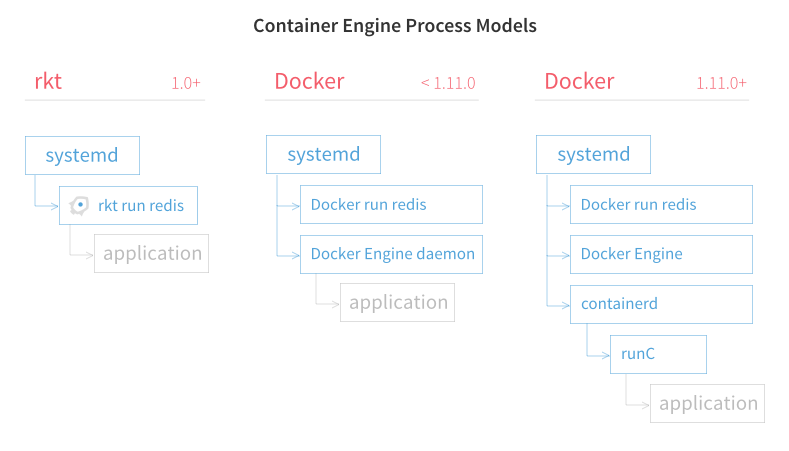
\includegraphics[scale=0.5]{img/rkt-vs-docker-process-model.png}
	\caption[Prozessmodelle im Vergleich zwischen rkt und Docker 
	\cite{imgrktvsdocker}]{Prozessmodelle im Vergleich zwischen rkt und 
		\texttt{docker} \cite{imgrktvsdocker}}
	\label{fig:rkt_vs_docker}
\end{figure}
Wo bei \texttt{rkt} ein Prozess direkt gestartet wird, wird er bei 
\texttt{docker} über eine Engine verwaltet. Die direkte Verwaltung hat den 
Vorteil, dass es eine Abstraktionsschicht weniger gibt. Die Engine bietet 
jedoch den Vorteil, dass man Containern die Möglichkeit gibt sich selbst oder 
sogar andere Container in der Engine zu verwalten, ohne dass man dabei zugriff 
auf das System geben muss. Die Abstraktionsebene kann also auch als 
Sicherheitslayer gesehen werden.\\
\\
Ein Vergleich zwischen \texttt{docker} und \texttt{railcar} fällt schwer, da es 
keine wirklichen Unterschiede dazwischen gibt. Nach Aussage eine Entwicklers 
von \texttt{railcar} sind die Laufzeitkomponenten zu 98\% 
identisch.\cite{railcarvsdocker} Des weiteren ist \texttt{railcar} nur ein 
drop-in für die Laufzeitkomponente von \ac{OCI} basierenden Applikationen.\\
\\
Die Wahl zum Tool für die Prozessvirtualisierung fällt somit auf 
\texttt{docker}. Dieses Tool ist bereits seit einigen Jahren im Einsatz und 
hierzu gibt es bereits viele Lösungen und Dokumentationen durch die Community. 
Des weiteren ist \texttt{docker} weiter verbreitet, weswegen die Unterstützung 
bei \acf{IaaS} und \acf{PaaS} Anbietern einfacher ist.
\subsection{Orchestrierung} \label{subsec:tunorch}
Anders wie die Werkzeuge zur Prozessvirtualisierung, gibt es für die in Kapitel 
\ref{subsec:sdtorch} genannten Tools (\texttt{docker swarm}, \texttt{ansible}, 
\texttt{puppet} und \texttt{kubernetes}) keinen Standard. Was jedoch schon beim 
lesen der Webseiten der Produkte auffällt, dass lediglich \texttt{kubernetes} 
direkt mit der Orchestrierung von Container-Engines wirbt.\\
\\
In der aktuellen Lösung \cite{osmib} werden \texttt{ansibile}-Skripte 
eingesetzt um die Container zu verwalten. Jedoch ist diese Lösung basiert auf 
einem einzelnen Container und müsste für die Orchestrierung stark erweitert 
werden. Die Mittel zur Container-Orchestrierung müssten hierbei selbst 
geschrieben werden, wie auch bei \texttt{puppet}.\cite{ansible}\cite{puppet}\\
\\
\texttt{docker swarm} bietet keine direkte Möglichkeit Orchestrierung zu 
betrieben. Anders wie \texttt{ansible} und \texttt{puppet} ist
\texttt{docker swarm} jedoch direkt in \texttt{docker} integriert und 
kommuniziert somit nativ mit der Container-Engine. Jedoch müssten auch hier die 
Werkzeuge zur Orchestrierung selbst geschrieben werden.\cite{dockSwarm}\\
\\
Unterschiedlich zu allen anderen genannten Werkzeugen bringt 
\texttt{kubernetes} sowohl alle Tools zur Verwaltung von Containern mit, aber 
auch alles um die Container zu orchestrieren. Es arbeitet eng mit der 
Container-Engine zusammen und man kann einfach von einem \texttt{docker swarm} 
dorthin migrieren, sodass auch eine lokale Entwicklung einfach 
fällt.\cite{kubernetes}\\
\\
Die Wahl zum Tool für die Orchestrierung fällt somit auf \texttt{docker swarm} 
und \texttt{kubernetes}. Auch in der Community und Wirtschaft gibt es für diese 
Lösung eine breite Unterstützung und \texttt{kubernetes} ist der de-facto 
Standard für das Orchesteriren von Applikationen. Hier bieten schon viele 
\ac{PaaS}-Anbieter ein \glqq{}\texttt{kubernetes}-as-a-Service\grqq{} an. Hier
können sich allerdings auch andere Tools ergeben, je nach Dienstleister oder
vom Kunden gewünschten verfahren können auch Technologien, wie z.B. 
CloudFoundry \cite{cloudfoundry} zum Einsatz kommen.
\section{Erwartetes Ergebnis}
%Wie bewerte ich das Ergebnis? 
Es wird eine Lösung erwartet, die ähnlich einfach bedienbar ist wie das 
momentane Multiinstace Backend \cite{osmib}. Man soll also Applikationen ohne 
Ausfallzeit updaten können. Wichtige Informationen über die Instanzen sollen 
schnell einsehbar sein. Die Container der Applikationen sollen agil und 
dynamisch auf Belastungen reagieren und skalieren.\\
\\
Kern der Anforderung ist es eine Lösung zu schaffen bei der, im Gegensatz zum 
momentanen Zustand, die Applikationen ohne administrativen Eingriff skalieren 
und dass Applikationen ohne Ausfallzeit updatebar sind. Dies soll zum einen dem 
Kunden Ausfälle und manuell auszugleichende Belastungsengpässe ersparen, aber 
auch kosten in der Administration sparen.\\
\\
Durch die automatische Skalierung und eine geschickte Planung von Terminen kann 
zudem auch die Leistung vorhandener Hardware besser genutzt werden, oder sogar 
in einem \ac{PPU} Modell angewendet werden. Dies sollte weiterhin die 
momentanen Kosten für einzel-Kunden senken.\\
\\
Ziel ist es die momentanen Zeitfaktoren in der Administration zu messen und 
diese mit den Zeitfaktoren nach der Entwicklung zu vergleichen. Des weiteren 
sollen die Kosten zur Bereitstellung verglichen werden. Erwartet wird, dass die 
Zeitfaktoren, vor allem durch die geringere Einzelbetreuung für eventuelle 
Belastungsspitzen deutlich sinken werden und das die kosten für die 
Bereitstellung für den einzelnen ebenfalls sinken.
\section{Planung}
%Zeitplan, Gantt-Diagramm o.Ä.
\begin{tabular}{l|p{13cm}}
	\textbf{Datum} & \textbf{Schritt} \\ \hline
	05.2018 & Anmeldung der Arbeit am Prüfungsamt \\
	20.06.2018 & Vortrag über die Arbeit im Oberseminar \\
	01-14.07.2018 & Verhindert an der Arbeit zu schreiben, da noch eine Klausur 
	in Informatik D geschrieben werden muss für den erfolgreichen Abschluss zum 
	Bachelor \\
	09.2018 & Abgabe der Arbeit\\
	09.2018 & Universitätspraktikum \\
	10.2018 & Abschluss mit Bachelor
\end{tabular}
\newpage
\section*{Akronyme}
\begin{acronym}[Bash]
	\acro{IaaS}{Infrastructure as a Service}
	\acro{PaaS}{Platform as a Service}
	\acro{SaaS}{Software as a Service}
	\acro{OCI}{Open Container Initiative}
	\acro{OSMIB}{OpenSlides Multiinstace Backend}
	\acro{PPU}{Pay per use}
\end{acronym}
\begin{thebibliography}{999}
	\bibitem {oshp} OpenSlides.org Homepage, \url{https://openslides.org/}, 
	abgerufen am 2018-03-15
	\bibitem {inte} Intevation GmbH Homepage, \url{http://intevation.de/}, 
	abgerufen am 2018-03-15
	\bibitem {gpg4win} Gpg4win Homepage, \url{https://www.gpg4win.de/}, 
	abgerufen am 2018-03-15
	\bibitem{djangohp} Django Homepage, \url{https://www.djangoproject.com/},
	abgerufen am 2018-04-11
	\bibitem{oscom} OpenSlides.com Homepage, \url{https://openslides.com/}, 
	abgerufen am 2018-03-15
	\bibitem{oci} Open Container Initiative, 
	\url{https://www.opencontainers.org/}, abgerufen am 2018-03-15
	\bibitem{containerhist} \glqq{}A Brief History of Containers: From 1970s 
	chroot to Docker 2016\grqq{}, von Rani Osnat, 05-05-2016 
	\url{https://blog.aquasec.com/a-brief-history-of-containers-from-1970s-chroo
	t-to-docker-2016},
	 abgerufen am 2018-03-15
	\bibitem{rkthp} CoreOS rkt Homepage, \url{https://coreos.com/rkt/}, 
	abgerufen am 2018-03-15
	\bibitem{railcarhp} RailCar GitHub Homepage, 
	\url{https://github.com/oracle/railcar}, abgerufen am 2018-03-15
	\bibitem{dockerhp} Docker Homepage, \url{https://www.docker.com/}, 
	abgerufen am 2018-03-15
	\bibitem{dockerdl} \glqq{}Docker's Tools of Mass Innovation: Explosive 
	Growth From Open-Source Containers to Commercial Platform for Modernizing 
	and Managing Apps\grqq{}, von Laura Bernheim, 2017-06-26, 
	\url{http://www.hostingadvice.com/blog/dockers-explosive-growth-from-open-so
	urce-containers-to-commercial-platform/},
	 abgerufen am 2018-03-15
	\bibitem{osmib} OpenSlides Multiinstance Backend GitHub Page, 
	\url{https://github.com/OpenSlides/openslides-multiinstance-backend}, 
	abgerufen am 2018-03-15
	\bibitem{osgh} OpenSlides Github Page, 
	\url{https://github.com/OpenSlides/OpenSlides}, abgerufen am 2018-03-15
	\bibitem{dockSwarm} Docker Swarm Homepage, 
	\url{https://docs.docker.com/engine/swarm/}, abgerufen am 2018-03-15
	\bibitem{kubernetes} Kubernetes Homepage, \url{https://kubernetes.io/}, 
	abgerufen am 2018-03-15
	\bibitem{puppet} Puppet Homepage, \url{https://puppet.com/}, abgerufen am 
	2018-03-15
	\bibitem{ansible} Ansible Homepage, \url{https://www.ansible.com/}, 
	abgerufen am 2018-03-15
	\bibitem{osdr} OpenSlides Docker Registry von emanuels, 
	\url{https://hub.docker.com/r/emanuels/openslides/builds/}, abgerufen am 
	2018-03-15
	\bibitem{rktvsdocker} \glqq{}Docker vs CoreOS Rkt\grqq{}, 08-09-2017, 
	\url{https://www.upguard.com/articles/docker-vs-coreos}, abgerufen am 
	2018-03-15
	\bibitem{imgrktvsdocker} \glqq{}rkt vs other projects\grqq{}, 
	\url{https://coreos.com/rkt/docs/latest/rkt-vs-other-projects.html}, 
	abgerufen am 2018-04-03
	\bibitem{railcarvsdocker} \glqq{}Oracle Releases an OCI-Based Container 
	Runtime\grqq{}, 05-07-2017 von Alex Handy,  
	\url{https://thenewstack.io/oracle-opens-oci-container-runtime/}, abgerufen 
	am 2018-04-03
	\bibitem{cloudfoundry}Cloud Foundry Website, 
	\url{https://www.cloudfoundry.org/}, abgerufen am 2018-04-09
	\bibitem{ocimembers} OCI Member Page ,
	\url{https://www.opencontainers.org/about/members},
	abgerufen am 2018-04-11
	\bibitem{nginx} ngix Website, \url{https://nginx.org/},
	abgerufen am 2018-04-11
	\bibitem{daphne} Daphne GitHub Repository, 
	\url{https://github.com/django/daphne/},
	abgerufen am 2018-04-11
	\bibitem{redis} Redis Website, \url{https://redis.io/},
	abgerufen am 2018-04-11
	\bibitem{postgres} Postgres Website, \url{https://www.postgresql.org/},
	abgerufen am 2018-04-11
\end{thebibliography}

\end{document}


